% !TEX encoding = UTF-8
% !TEX TS-program = pdflatex
% !TEX root = ../Tesi.tex

%************************************************

%************************************************
Segue un overview delle fonti dati da cui è possibile costruire una argumentation framework da dibattiti.

\section {Twitter} %%%%%%%%%%%%%%%%%%%%%%%%%%%%%%%%%%%%%%%%%%%

Lo scraping del sito Web è vietata dal Twitter Terms of Service, quindi l'unico modo rimane l'accesso tramite API. Per accedere alla piattaforma delle API di twitter è necessario creare un Twitter developer account ed in seguito creare dal portale una applicazione nella quale si dichiara lo scopo dello dell'accesso ai contenuti e si richiedono i relativi permessi. Una volta ottenuta l'approvazione, vengono rilasciati delle credenziali per l'autenticazione agli endpoint. I contenuti messi a disposizione sono i Tweet pubblici e le risposte cercando parole chiave specifiche attraverso le Search API o chiedendo esempi di Tweet a determinati account attraverso le User API. Inoltre è possibile richiedere tweet specifici conoscendone l'id.

\subsection {Overview}

Il problema è che al momento non è disponibile l'accesso alle conversazioni ed inoltre la richiesta di tweet tramite le Search API o le User API restituisce solo un sottoinsieme dei tweet, questo rende difficile cercare di ricostruire le conversazioni dai tweet restituiti dalla query.

\subsubsection {Ricostruire la conversazione} 
\label{ricostruire-conv}
Fra gli attributi presenti nei tweet è presente il campo \textbf{"in reply to status id"} che, se presente, contiene l'id del tweet al quale il tweet corrente sta rispondendo. Questo può essere utilizzato per cercare di ricostruire la conversazione, facendo una altra richiesta tramite API per avere il tweet risposto. Per qualsiasi tweet con questo campo, possiamo:
\begin{itemize}
    \item trovare il tweet a cui quello corrente sta rispondendo, quindi ripetere la procedura per ogni tweet con questo attributo avvalorato in modo da ottenere delle sequenze di tweet.
    \item Una volta create le sequenze di tweet, se queste contengono elementi in comune, unire le sequenze creando un grafo della conversazione.
    \item Valutare la bontà del grafo ottenuto mediante euristiche come il numero di elementi (tweet) nel grafo, o la presenza di diramazioni, ovvero nodi più archi in entrata.
\end{itemize}

Quindi costruire grafo orientato della conversazione $\mathcal{G = ⟨V, E⟩}$, dove i nodi $v \in \mathcal{V}$ sono tweet ed esiste un arco $(v_1,v_2) \in \mathcal{E}$ se l'attributo \textbf{"in reply to status id"} di $v_1$ contiene l'id di $v_2$.

Tuttavia le API forniscono l'accesso solo ad un campione dei tweet, quindi potrebbe non essere possibile recuperare dei tweet quando si tenta di ricostruire la conversazione. Un'altra limitazione proviene dal numero di tweet iniziale che è possibile ottenere in risposta alla query, che risulta essere massimo 1000, dei quali è necessario filtrare i tweet che contengono il campo \textbf{"in reply to status id"} avvalorato, numero che può variare di molto (di solito circa il 10\%). Inoltre le conversazioni risultano quasi sempre essere sequenze lineari di nodi, ovvero grafi con archi in entrata $\leq 1$ ed archi in uscita $\leq 1$ come rappresentato in figura \ref{fig:comment-twitter}. Inoltre il grafo ricostruito cambia in base a quando si fa la richiesta tramite API.

\begin{figure}[ht]
    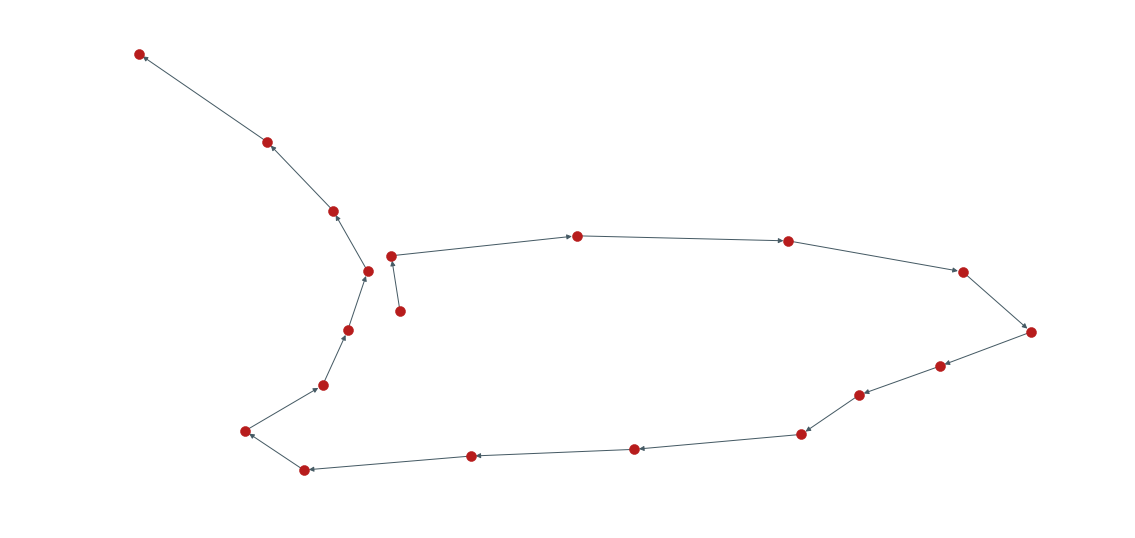
\includegraphics[width=\linewidth]{Immagini/twitter.png}
    \caption{Rappresentazione del grafo della conversazione, utilizzando come nodi i commenti.}
    \label{fig:comment-twitter}
\end{figure}

\subsubsection {Utenti come nodi}
Un altro approccio utilizzato, indipendente dalle funzionalità messe a disposizione da Twitter o dalle Twitter API, consiste nel considerare gli utenti in una conversazione come nodi e creare un arco orientato tra due utenti se esiste almeno un tweet di risposta tra i due, più formalmente: costruire un grafo orientato $\mathcal{G = ⟨V, E⟩}$, dove i nodi $v \in \mathcal{V}$ sono utenti ed esiste un arco $(v_1,v_2) \in \mathcal{E}$ se esiste almeno un tweet con utente $v_1$ e con l'attributo \textbf{"in reply to status id"} contenente l'id di un tweet appartenente all'utente $v_2$.

Anche qui si presentano i problemi presentati nella sezione precedente \ref{ricostruire-conv}, tuttavia il grafo risultante presenta nodi con archi in entrata $\geq 1$ ed archi in uscita $\geq 1$, come rappresentato in figura \ref{fig:users-twitter}.

\begin{figure}[ht]
    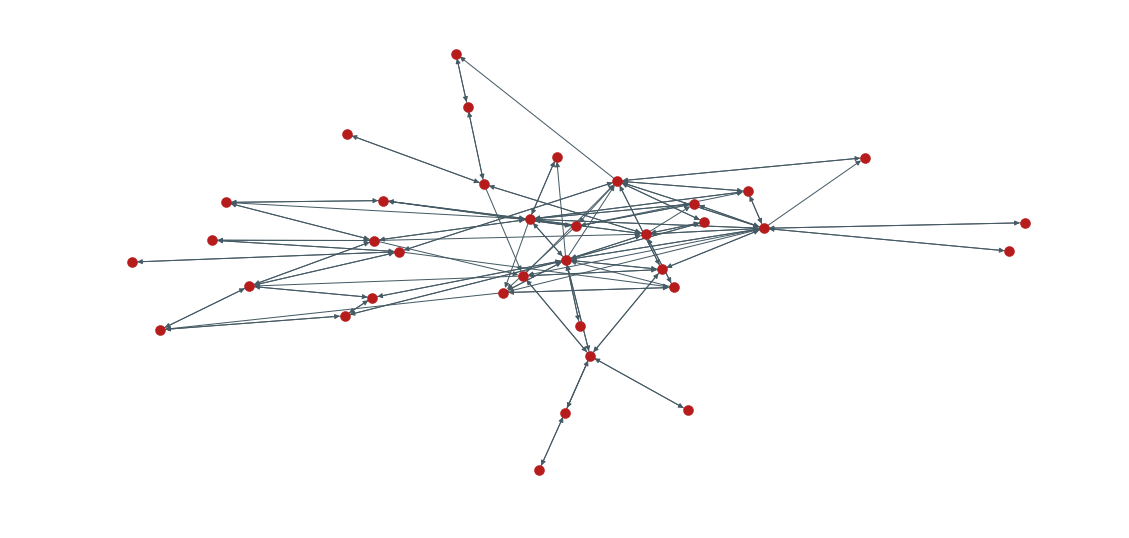
\includegraphics[width=\linewidth]{Immagini/twitter-users.png}
    \caption{Rappresentazione del grafo della conversazione, utilizzando come nodi gli utenti.}
    \label{fig:users-twitter}
\end{figure}



%%%%%%%%%%%%%%%%%%%%%%%%%%%%%%%%%%%%%%%%%%%%%%%%%%%%%%%%%%%%%%%
%%%%%%%%%%%%%%%%%%%%%%%%%%%%%%%%%%%%%%%%%%%%%%%%%%%%%%%%%%%%%%%
%%%%%%%%%%%%%%%%%%%%%%%%%%%%%%%%%%%%%%%%%%%%%%%%%%%%%%%%%%%%%%%
%%%%%%%%%%%%%%%%%%%%%%%%%%%%%%%%%%%%%%%%%%%%%%%%%%%%%%%%%%%%%%%
%%%%%%%%%%%%%%%%%%%%%%%%%%%%%%%%%%%%%%%%%%%%%%%%%%%%%%%%%%%%%%%


\section {Stackoverflow} %%%%%%%%%%%%%%%%%%%%%%%%%%%%%%%%%%%%%%%%%%%

\begin{itemize}
    \item create account at https://stackapps.com/
    \item register an app
    \item b
\end{itemize}

\subsection {Overview}
\subsubsection {API}

\subsubsection {Commenti}
\subsubsection {Utenti}


%%%%%%%%%%%%%%%%%%%%%%%%%%%%%%%%%%%%%%%%%%%%%%%%%%%%%%%%%%%%%%%
%%%%%%%%%%%%%%%%%%%%%%%%%%%%%%%%%%%%%%%%%%%%%%%%%%%%%%%%%%%%%%%
%%%%%%%%%%%%%%%%%%%%%%%%%%%%%%%%%%%%%%%%%%%%%%%%%%%%%%%%%%%%%%%
%%%%%%%%%%%%%%%%%%%%%%%%%%%%%%%%%%%%%%%%%%%%%%%%%%%%%%%%%%%%%%%
%%%%%%%%%%%%%%%%%%%%%%%%%%%%%%%%%%%%%%%%%%%%%%%%%%%%%%%%%%%%%%%

\section {Reddit} %%%%%%%%%%%%%%%%%%%%%%%%%%%%%%%%%%%%%%%%%%%

\subsection {Overview}
\subsubsection {API}

\subsubsection {Commenti}
\subsubsection {Utenti}

% Fatti generati argument/1, attac- k/2, support/2, rel_weight/3

% descrizione vader e altri componenti utilizzati

